\documentclass[tikz,border=8pt]{standalone}
% Shared look for every TikZ diagram. Load with % Shared look for every TikZ diagram. Load with % Shared look for every TikZ diagram. Load with \input{../../tools/tikz-style.tex}
\usepackage[T1]{fontenc}
\usepackage{lmodern}
\renewcommand{\sfdefault}{lmr}  % diagrams use the same serif as the text
\usetikzlibrary{arrows.meta, positioning, shapes.geometric, calc, fit, backgrounds}
\definecolor{cblue}{HTML}{4C78A8}
\definecolor{corange}{HTML}{F58518}
\definecolor{cgreen}{HTML}{54A24B}
\definecolor{cred}{HTML}{E45756}
\definecolor{cpurple}{HTML}{B279A2}
\definecolor{cgrey}{HTML}{6B6B6B}
\tikzset{
  every picture/.style={font=\sffamily, line width=1.2pt},
  box/.style={draw=#1, fill=#1!12, rounded corners=4pt, align=center, inner sep=7pt, minimum height=1.1cm},
  box/.default=cgrey,
  arrow/.style={-{Stealth[length=3mm]}, draw=cgrey, line width=1.4pt},
  title/.style={font=\sffamily\bfseries\Large},
  note/.style={font=\sffamily\small, text=cgrey, align=center},
}
\AtBeginDocument{\hyphenpenalty=10000 \exhyphenpenalty=10000}

\usepackage[T1]{fontenc}
\usepackage{lmodern}
\renewcommand{\sfdefault}{lmr}  % diagrams use the same serif as the text
\usetikzlibrary{arrows.meta, positioning, shapes.geometric, calc, fit, backgrounds}
\definecolor{cblue}{HTML}{4C78A8}
\definecolor{corange}{HTML}{F58518}
\definecolor{cgreen}{HTML}{54A24B}
\definecolor{cred}{HTML}{E45756}
\definecolor{cpurple}{HTML}{B279A2}
\definecolor{cgrey}{HTML}{6B6B6B}
\tikzset{
  every picture/.style={font=\sffamily, line width=1.2pt},
  box/.style={draw=#1, fill=#1!12, rounded corners=4pt, align=center, inner sep=7pt, minimum height=1.1cm},
  box/.default=cgrey,
  arrow/.style={-{Stealth[length=3mm]}, draw=cgrey, line width=1.4pt},
  title/.style={font=\sffamily\bfseries\Large},
  note/.style={font=\sffamily\small, text=cgrey, align=center},
}
\AtBeginDocument{\hyphenpenalty=10000 \exhyphenpenalty=10000}

\usepackage[T1]{fontenc}
\usepackage{lmodern}
\renewcommand{\sfdefault}{lmr}  % diagrams use the same serif as the text
\usetikzlibrary{arrows.meta, positioning, shapes.geometric, calc, fit, backgrounds}
\definecolor{cblue}{HTML}{4C78A8}
\definecolor{corange}{HTML}{F58518}
\definecolor{cgreen}{HTML}{54A24B}
\definecolor{cred}{HTML}{E45756}
\definecolor{cpurple}{HTML}{B279A2}
\definecolor{cgrey}{HTML}{6B6B6B}
\tikzset{
  every picture/.style={font=\sffamily, line width=1.2pt},
  box/.style={draw=#1, fill=#1!12, rounded corners=4pt, align=center, inner sep=7pt, minimum height=1.1cm},
  box/.default=cgrey,
  arrow/.style={-{Stealth[length=3mm]}, draw=cgrey, line width=1.4pt},
  title/.style={font=\sffamily\bfseries\Large},
  note/.style={font=\sffamily\small, text=cgrey, align=center},
}
\AtBeginDocument{\hyphenpenalty=10000 \exhyphenpenalty=10000}

\begin{document}
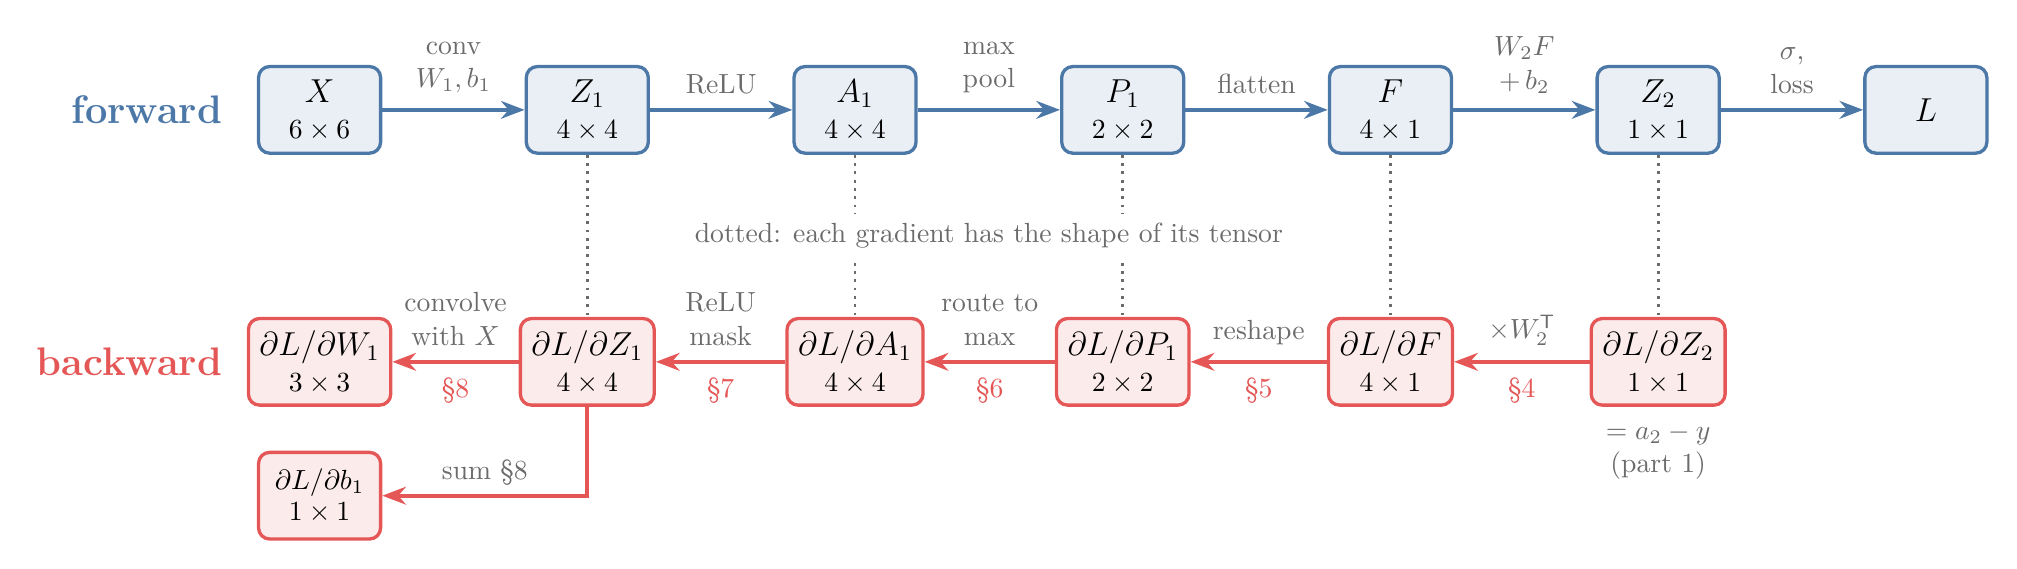
\begin{tikzpicture}[t/.style={box=cblue, minimum width=1.55cm, inner sep=4pt, font=\sffamily\large},
                    g/.style={box=cred, minimum width=1.55cm, inner sep=4pt, font=\sffamily\large},
                    op/.style={font=\sffamily\normalsize, text=cgrey, align=center}]
  \def\dx{3.4}
  % forward row
  \foreach \n/\s [count=\i from 0] in {X/6\times6, Z_1/4\times4, A_1/4\times4, P_1/2\times2, F/4\times1, Z_2/1\times1}
    \node[t] (f\i) at (\i*\dx,0) {$\n$\\[-1pt]{\normalsize $\s$}};
  \node[t] (f6) at (6*\dx,0) {$L$};
  \foreach \a/\b/\o in {0/1/{conv\\$W_1, b_1$}, 1/2/ReLU, 2/3/{max\\pool}, 3/4/flatten, 4/5/{$W_2F$\\$+\,b_2$}, 5/6/{$\sigma$,\\loss}}
    \draw[arrow, draw=cblue] (f\a) -- node[op, above=2pt] {\o} (f\b);
  \node[title, anchor=east, text=cblue] at (-1.1,0) {forward};
  % backward row
  \node[g] (b0) at (0,-3.2) {$\partial L/\partial W_1$\\[-1pt]{\normalsize $3\times3$}};
  \node[g, font=\sffamily\normalsize] (bb) at (0,-4.9) {$\partial L/\partial b_1$\\[-1pt]{$1\times1$}};
  \foreach \n/\s [count=\i from 1] in {Z_1/4\times4, A_1/4\times4, P_1/2\times2, F/4\times1, Z_2/1\times1}
    \node[g] (b\i) at (\i*\dx,-3.2) {$\partial L/\partial \n$\\[-1pt]{\normalsize $\s$}};
  \node[op, below=2pt of b5] {$=a_2-y$\\(part 1)};
  \foreach \a/\b/\o/\sec in {5/4/{$\times W_2^{\mathsf T}$}/4, 4/3/reshape/5, 3/2/{route to\\max}/6, 2/1/{ReLU\\mask}/7, 1/0/{convolve\\with $X$}/8}
    \draw[arrow, draw=cred] (b\a) -- node[op, above=2pt] {\o} node[op, below=2pt, text=cred] {\S\sec} (b\b);
  \draw[arrow, draw=cred] (b1.south) |- node[op, pos=0.75, above] {sum \S8} (bb.east);
  \node[title, anchor=east, text=cred] at (-1.1,-3.2) {backward};
  % same shapes
  \foreach \i in {1,...,5} \draw[cgrey, dotted, line width=1pt] (f\i.south) -- (b\i.north);
  \node[op, fill=white] at (8.5,-1.6) {dotted: each gradient has the shape of its tensor};
\end{tikzpicture}
\end{document}
